
\section{Satelliten}
\label{section:satelliten}
\begin{frame}%STARTCONTENT

\begin{columns}
    \begin{column}{0.48\textwidth}
    
\begin{figure}
    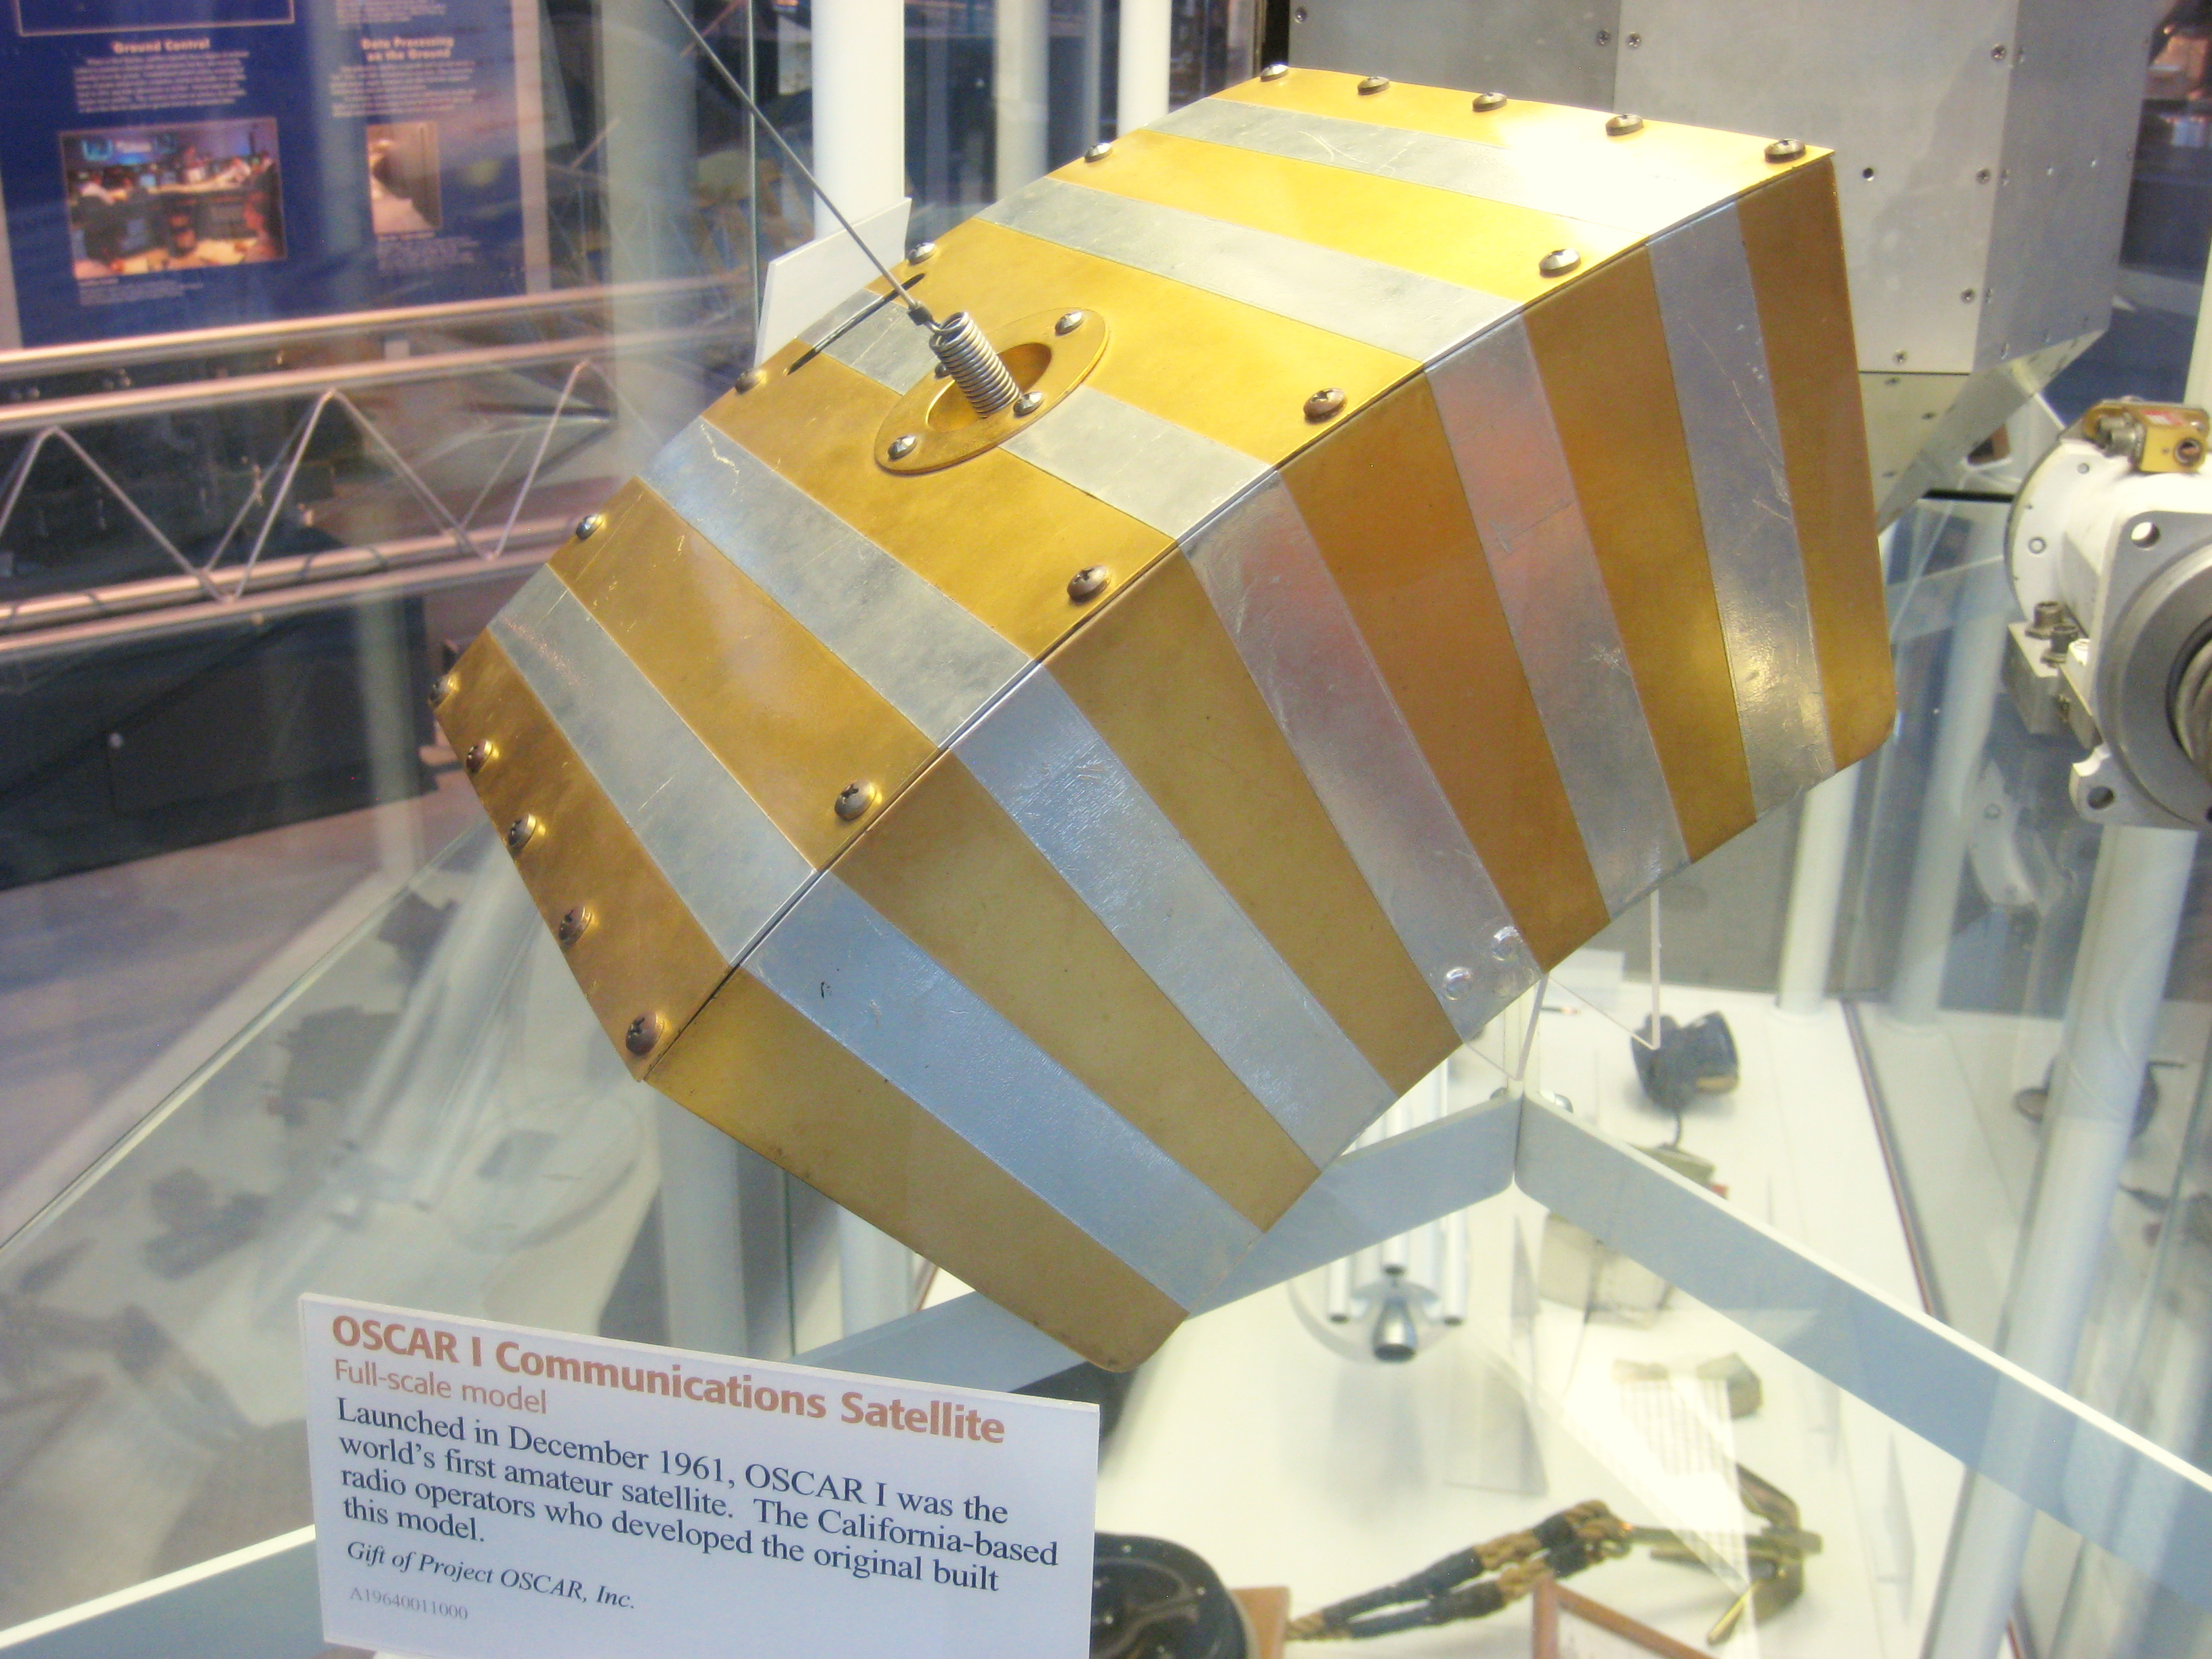
\includegraphics[width=0.85\textwidth]{foto/124}
    \caption{\scriptsize Modell des ersten Amateurfunksatelliten OSCAR 1, der 1961 für 22 Tage aus dem Orbit der Erde eine Bake im \qty{2}{\metre}-Band sendete und von 570 Funkamateuren aus 28 Ländern gehört wurde}
    \label{n_satellit_oscar1}
\end{figure}

    \end{column}
   \begin{column}{0.48\textwidth}
       \begin{itemize}
  \item Umrunden die Erde in kreis- oder elliptischen Bahnen und in unterschiedlichen Höhen
  \item Erster Amateurfunksatellit bereits 1961 (OSCAR 1)
  \item OSCAR: \enquote{Orbiting Satellite Carrying Amateur Radio}
  \item Bis heute mehrere 100 Satelliten im Orbit (gewesen)
  \end{itemize}

   \end{column}
\end{columns}

\end{frame}

\begin{frame}
\only<1>{
\begin{QQuestion}{BE415}{Wofür steht die Abkürzung OSCAR im Amateurfunk?}{Fahrzeug mit betriebsbereiter Amateurfunkstelle (Operational Station on a CAR)}
{Schiff auf See mit Amateurfunkstelle (Offshore Ship Carrying Amateur Radio)}
{Satellit mit Amateurfunkstelle (Orbiting Satellite Carrying Amateur Radio)}
{Amateurfunkstelle im Luftradarbetrieb (Observation Station Conducting Aeronautical Radar)}
\end{QQuestion}

}
\only<2>{
\begin{QQuestion}{BE415}{Wofür steht die Abkürzung OSCAR im Amateurfunk?}{Fahrzeug mit betriebsbereiter Amateurfunkstelle (Operational Station on a CAR)}
{Schiff auf See mit Amateurfunkstelle (Offshore Ship Carrying Amateur Radio)}
{\textbf{\textcolor{DARCgreen}{Satellit mit Amateurfunkstelle (Orbiting Satellite Carrying Amateur Radio)}}}
{Amateurfunkstelle im Luftradarbetrieb (Observation Station Conducting Aeronautical Radar)}
\end{QQuestion}

}
\end{frame}

\begin{frame}
\frametitle{Transponder}
Relaisfunkstelle auf dem Satellit wird \enquote{Transponder} genannt
\begin{columns}
    \begin{column}{0.48\textwidth}
    Uplink: Funkstrecke von der Erde zum Satelliten


    \end{column}
   \begin{column}{0.48\textwidth}
       Downlink: Funkstrecke vom Satelliten zur Erde


   \end{column}
\end{columns}

\begin{itemize}
  \item Unterschiedliche Frequenzbänder für Up- und Downlink
  \item Einfachere Trennung von Sende- und Empfangssignal
  \item Baugröße von Filtern wird reduziert
  \end{itemize}

\end{frame}

\begin{frame}
\only<1>{
\begin{QQuestion}{BE416}{Was versteht man unter dem Transponder eines \glqq OSCAR\grqq{} und wie arbeitet er?}{Dies ist ein Umsetzer an Bord eines Amateurfunksatelliten, der die aufgenommenen Signale in einen anderen Frequenzbereich umsetzt und wieder zur Erde sendet.}
{Es handelt sich um einen mit einer fernbedienten Amateurfunkstelle bestückten Stratosphärenballon, der empfangene Signale aufbereitet zur Erde zurücksendet.}
{Dies ist ein Umsetzer an Bord eines Amateurfunksatelliten, der die vom Satelliten aufgenommenen Wetterbilder und weitere Telemetriedaten automatisch zur Erde sendet.}
{Dies ist ein Bakensender an Bord eines Amateurfunksatelliten, der zur Beobachtung der Ausbreitungsbedingungen im VHF-, UHF- und SHF-Bereich dient.}
\end{QQuestion}

}
\only<2>{
\begin{QQuestion}{BE416}{Was versteht man unter dem Transponder eines \glqq OSCAR\grqq{} und wie arbeitet er?}{\textbf{\textcolor{DARCgreen}{Dies ist ein Umsetzer an Bord eines Amateurfunksatelliten, der die aufgenommenen Signale in einen anderen Frequenzbereich umsetzt und wieder zur Erde sendet.}}}
{Es handelt sich um einen mit einer fernbedienten Amateurfunkstelle bestückten Stratosphärenballon, der empfangene Signale aufbereitet zur Erde zurücksendet.}
{Dies ist ein Umsetzer an Bord eines Amateurfunksatelliten, der die vom Satelliten aufgenommenen Wetterbilder und weitere Telemetriedaten automatisch zur Erde sendet.}
{Dies ist ein Bakensender an Bord eines Amateurfunksatelliten, der zur Beobachtung der Ausbreitungsbedingungen im VHF-, UHF- und SHF-Bereich dient.}
\end{QQuestion}

}
\end{frame}

\begin{frame}
\only<1>{
\begin{QQuestion}{BE411}{Was bedeutet der Begriff Uplink im Bereich der Satellitenkommunikation?}{Senderichtung vom Satelliten zur Erde}
{Senderichtung von der Erde zum Satelliten}
{Horizontaler Winkel der Antenne}
{Vertikaler Winkel der Antenne}
\end{QQuestion}

}
\only<2>{
\begin{QQuestion}{BE411}{Was bedeutet der Begriff Uplink im Bereich der Satellitenkommunikation?}{Senderichtung vom Satelliten zur Erde}
{\textbf{\textcolor{DARCgreen}{Senderichtung von der Erde zum Satelliten}}}
{Horizontaler Winkel der Antenne}
{Vertikaler Winkel der Antenne}
\end{QQuestion}

}
\end{frame}

\begin{frame}
\only<1>{
\begin{QQuestion}{BE412}{Was bedeutet der Begriff Downlink im Bereich der Satellitenkommunikation?}{Senderichtung vom Satelliten zur Erde}
{Senderichtung von der Erde zum Satelliten}
{Horizontaler Winkel der Antenne}
{Vertikaler Winkel der Antenne}
\end{QQuestion}

}
\only<2>{
\begin{QQuestion}{BE412}{Was bedeutet der Begriff Downlink im Bereich der Satellitenkommunikation?}{\textbf{\textcolor{DARCgreen}{Senderichtung vom Satelliten zur Erde}}}
{Senderichtung von der Erde zum Satelliten}
{Horizontaler Winkel der Antenne}
{Vertikaler Winkel der Antenne}
\end{QQuestion}

}
\end{frame}

\begin{frame}
\only<1>{
\begin{QQuestion}{NF113}{Warum befinden sich bei Satellitenbetrieb Up- und Downlink in der Regel nicht im gleichen Frequenzband? Man benutzt unterschiedliche Frequenzbänder, weil~...}{der Uplink durch die Ionosphäre stärker bedämpft wird als der Downlink.}
{dies eine einfachere Trennung von Sende- und Empfangssignal ermöglicht und die Baugröße von Filtern auf dem Satelliten reduziert wird.}
{die Bandbreite auf beiden Frequenzbändern aufgeteilt wird und Bandbereiche besser ausgenutzt werden können. }
{man damit den Dopplereffekt vermindert.}
\end{QQuestion}

}
\only<2>{
\begin{QQuestion}{NF113}{Warum befinden sich bei Satellitenbetrieb Up- und Downlink in der Regel nicht im gleichen Frequenzband? Man benutzt unterschiedliche Frequenzbänder, weil~...}{der Uplink durch die Ionosphäre stärker bedämpft wird als der Downlink.}
{\textbf{\textcolor{DARCgreen}{dies eine einfachere Trennung von Sende- und Empfangssignal ermöglicht und die Baugröße von Filtern auf dem Satelliten reduziert wird.}}}
{die Bandbreite auf beiden Frequenzbändern aufgeteilt wird und Bandbereiche besser ausgenutzt werden können. }
{man damit den Dopplereffekt vermindert.}
\end{QQuestion}

}
\end{frame}

\begin{frame}
\frametitle{Azimut und Elevation}
Satellitenantennen müssen ausgerichtet sein
\begin{columns}
    \begin{column}{0.48\textwidth}
    Azimut

\begin{itemize}
  \item stammt von arabisch السموت (as-sumūt, \enquote{die Wege})
  \item Richtung entlang des Horizonts
  \item Wird wie beim Kompass in Grad gemessen
  \item \qty{0}{\degree}/\qty{360}{\degree} Norden – \qty{90}{\degree} Osten – \qty{180}{\degree} Süden – \qty{270}{\degree} Westen
  \end{itemize}

    \end{column}
   \begin{column}{0.48\textwidth}
       Elevation

\begin{itemize}
  \item leitet sich von lateinisch elevare (\enquote{erheben}) ab
  \item Vertikaler Winkel über dem Horizont
  \item \qty{0}{\degree} $\rightarrow$ direkt am Horizont
  \item \qty{90}{\degree} $\rightarrow$ senkrecht über einem
  \end{itemize}

   \end{column}
\end{columns}

\end{frame}

\begin{frame}
\only<1>{
\begin{QQuestion}{BE413}{Was bedeutet der Begriff Azimut im Bereich der Satellitenkommunikation?}{Vertikaler Winkel der Antenne}
{Horizontaler Winkel der Antenne}
{Senderichtung vom Satelliten zur Erde}
{Senderichtung von der Erde zum Satelliten}
\end{QQuestion}

}
\only<2>{
\begin{QQuestion}{BE413}{Was bedeutet der Begriff Azimut im Bereich der Satellitenkommunikation?}{Vertikaler Winkel der Antenne}
{\textbf{\textcolor{DARCgreen}{Horizontaler Winkel der Antenne}}}
{Senderichtung vom Satelliten zur Erde}
{Senderichtung von der Erde zum Satelliten}
\end{QQuestion}

}
\end{frame}

\begin{frame}
\only<1>{
\begin{QQuestion}{BE414}{Was bedeutet der Begriff Elevation im Bereich der Satellitenkommunikation?}{Horizontaler Winkel der Antenne}
{Vertikaler Winkel der Antenne}
{Senderichtung vom Satelliten zur Erde}
{Senderichtung von der Erde zum Satelliten}
\end{QQuestion}

}
\only<2>{
\begin{QQuestion}{BE414}{Was bedeutet der Begriff Elevation im Bereich der Satellitenkommunikation?}{Horizontaler Winkel der Antenne}
{\textbf{\textcolor{DARCgreen}{Vertikaler Winkel der Antenne}}}
{Senderichtung vom Satelliten zur Erde}
{Senderichtung von der Erde zum Satelliten}
\end{QQuestion}

}
\end{frame}

\begin{frame}
\frametitle{Steuersignale}
\begin{itemize}
  \item Im Amateurfunkdienst gibt es eine Pflicht zur offenen Sprache
  \item Ausnahme: Steuersignale zwischen Bodenstationen und Amateurfunksatelliten
  \item Dürfen zum Zwecke der Verschleierung verschlüsselt werden
  \item Damit können Dritte die Signale nicht mitlesen
  \item Dient der Sicherheit der Satelliten vor Steuerkommandos von Unbefugten
  \item In Deutschland gilt das auch für automatische und fernbediente Stationen sowie Remote-Stationen
  \end{itemize}
\end{frame}

\begin{frame}
\only<1>{
\begin{QQuestion}{VA303}{Welche Kommunikationsinhalte dürfen im internationalen Amateurfunkverkehr laut Radio Regulations (RR) zum Zwecke der Verschleierung verschlüsselt werden?}{Vertrauliche Informationen und Mitteilungen persönlicher Art}
{Steuersignale zwischen Bodenkontrollstationen auf der Erde und Amateurfunksatelliten}
{Inhalte, die auf Grund des verwendeten Übertragungsverfahrens digital codiert werden}
{Inhalte, die schützenswerte technische Sachverhalte des Amateurfunkdienstes betreffen}
\end{QQuestion}

}
\only<2>{
\begin{QQuestion}{VA303}{Welche Kommunikationsinhalte dürfen im internationalen Amateurfunkverkehr laut Radio Regulations (RR) zum Zwecke der Verschleierung verschlüsselt werden?}{Vertrauliche Informationen und Mitteilungen persönlicher Art}
{\textbf{\textcolor{DARCgreen}{Steuersignale zwischen Bodenkontrollstationen auf der Erde und Amateurfunksatelliten}}}
{Inhalte, die auf Grund des verwendeten Übertragungsverfahrens digital codiert werden}
{Inhalte, die schützenswerte technische Sachverhalte des Amateurfunkdienstes betreffen}
\end{QQuestion}

}
\end{frame}

\begin{frame}
\only<1>{
\begin{QQuestion}{VD104}{Welche Kommunikationsinhalte dürfen im Amateurfunkverkehr laut AFuV zum Zwecke der Verschleierung verschlüsselt werden?}{Inhalte, die auf Grund des verwendeten Übertragungsverfahrens digital codiert werden}
{Steuersignale für Satelliten, vertrauliche Informationen und Mitteilung persönlicher Art}
{Steuersignale für Satelliten, für fernbediente und automatisch arbeitende Stationen und für Remote-Betrieb}
{Inhalte, die schützenswerte technische Sachverhalte des Amateurfunkdienstes betreffen}
\end{QQuestion}

}
\only<2>{
\begin{QQuestion}{VD104}{Welche Kommunikationsinhalte dürfen im Amateurfunkverkehr laut AFuV zum Zwecke der Verschleierung verschlüsselt werden?}{Inhalte, die auf Grund des verwendeten Übertragungsverfahrens digital codiert werden}
{Steuersignale für Satelliten, vertrauliche Informationen und Mitteilung persönlicher Art}
{\textbf{\textcolor{DARCgreen}{Steuersignale für Satelliten, für fernbediente und automatisch arbeitende Stationen und für Remote-Betrieb}}}
{Inhalte, die schützenswerte technische Sachverhalte des Amateurfunkdienstes betreffen}
\end{QQuestion}

}
\end{frame}%ENDCONTENT
